\documentclass[11pt,english,french]{scrreprt}
\usepackage{lmodern}
\usepackage{babel}
\renewcommand{\familydefault}{\rmdefault}
\usepackage[T1]{fontenc}
\usepackage{ucs}
\usepackage[utf8x]{inputenc}
\usepackage[a4paper]{geometry}
\geometry{verbose,tmargin=2cm,bmargin=2cm,lmargin=2cm,rmargin=2cm,headheight=2cm,footskip=1cm}
\setlength{\parskip}{\smallskipamount}
\setlength{\parindent}{0pt}

\usepackage{amsthm}
\usepackage{booktabs}
\usepackage{amsmath}
\usepackage[unicode=true, pdfusetitle,
 bookmarks=true,bookmarksnumbered=false,bookmarksopen=false,
 breaklinks=false,pdfborder={0 0 1},backref=false,colorlinks=false]
 {hyperref}

\makeatletter
\usepackage{colortbl}
\usepackage{color}
\usepackage[dvipsnames]{xcolor}
\usepackage{wrapfig}
\usepackage{graphicx}
\usepackage{listings}
\usepackage[calcwidth]{titlesec}
\usepackage{fix-cm}
\usepackage{multicol}
\usepackage{verbatim}
\usepackage{moreverb}
\usepackage{nicefrac}
\usepackage{amssymb}
\usepackage{array}
\usepackage{tabularx}
\usepackage{subfig}

\theoremstyle{remark}
  \newtheorem*{rem*}{Remarque}
\theoremstyle{definition}
  \newtheorem*{defi}{Définition}
  \newtheorem{ques}{Question}[section]

\definecolor{MyDarkBlue}{rgb}{0,0.08,0.45}

\lstset{language=C,
	 	basicstyle=\small\ttfamily,
		keywordstyle=\small\ttfamily,
		identifierstyle=,
		commentstyle=\textcolor{OliveGreen},
		columns=fullflexible,
		stringstyle=\small\ttfamily,
		showstringspaces=false,numberstyle=\tiny, breaklines=false, tabsize=4}

\titleformat{\section}[hang]{\sffamily\bfseries}
 {\Large\thesection}{12pt}{\Large}[{\titlerule[0.5pt]}]

\def\thickhrulefill{\leavevmode \leaders \hrule height 1pt\hfill \kern \z@}
\renewcommand{\maketitle}{\begingroup%
    \let\footnotesize\small
    \let\footnoterule\relax
    \parindent \z@
    \reset@font
    \begin{flushleft}
      \huge \sffamily \bfseries\color{orange} \@title
    \end{flushleft}
    \hrule height 1pt
    \begin{flushright}
      \large\sffamily\color{MyDarkBlue}\@author
    \end{flushright}
  \endgroup%
  \setcounter{footnote}{0}%
}

\AtBeginDocument{
  \def\labelitemi{\normalfont\bfseries{--}}
}

\makeatletter
\renewcommand\thesection{\arabic{section}}
\@addtoreset{section}{chapter}
\makeatother

\makeatother
\begin{document}
	
\title{LI310 - Examen 2009\\
Vendredi 4 janvier 2010}
\author{Benjamin BARON}

\maketitle

\section{Transmission de données} % (fold)

\begin{ques}
	Loi de Shannon :
	\[
		C_b = B_c\log_2(1+\frac{P_S}{P_N})\Leftrightarrow B_c = \frac{C_b}{\log_2(1+\frac{P_S}{P_N})}
	\]

	Or \[\frac{P_S}{P_N}=10^{\frac{\nicefrac{S}{N}}{10}}=10^{\frac{9,15}{10}}\approx 8,22\]

	Application numérique : \[B_c=\frac{2.10^6}{\log_2(1+8,22)}=6,24.10^5 \;\textrm{Hz}\]
	Nombre de canaux : \[n=\frac{1.10^6}{6,24.10^5}\approx 16,0257\]

	On pourra alors constituer au maximum $n=16$ canaux de bande passante 624 kHz.
\end{ques}

\begin{ques}
	Loi de Nyquist :\[D\leqslant 2B\log_2(M)\Leftrightarrow M\geqslant 2^{\frac{D}{2B}}\]
	
	Application numérique : \[M\geqslant 2^{\frac{2.10^6}{2\times 800.10^3}}\approx 2,378\]
	Ainsi, $M=4$. Il s'agit donc d'un code NRZ 4-aire.
	
	Durée $T_S$ de chacun des symboles : \[T_S = \frac{\log_2(M)}{D_b}\]
	Application numérique : \[T_S = \frac{\log_2(4)}{2.10^6}=1.10^{-6}\;\textrm{s} = 1\;\mu\textrm{s}\]
\end{ques}

\begin{ques}
	Voie BV à 4 Mbit/s. Solution permettant de garder les mêmes paramètres.\\
	Puisque c'est du multiplexage fréquentiel, alors on peut regrouper deux voies BV de 2 Mbits/s en une voie voie BV de 4 Mibt/s (ou allouer deux canaux BV à une seule BV). Il y aura donc : \begin{itemize}
		\item Une voie BV de 4 Mbit/s;
		\item 10 voies BV de 2 Mbit/s.
	\end{itemize}
	
	Solution qui permette d'offrir 12 voies BV dont une à 4 Mbit/s en modifiant les paramètres de codage de l'un des canaux.\\
	En modifiant les paramètres de codage de l'un des canaux, on a alors :\[M\geqslant 2^{\frac{4.10^6}{2\times 800.10^3}}\approx 5,657\]
	Donc en prenant $M=8$, on a bien le résultat souhaité. De plus, la durée $T_S$ de chacun des symboles sera de \[T_S=\frac{\log(8)}{4.10^6} = 7,5.10^{-7}\;\textrm{s}=0,75\;\mu\textrm{s}\]
\end{ques}

\section{HDLC} % (fold)

\begin{ques}\hfill
	
	\begin{tabularx}{\textwidth}{lX}
		Source & \lstinline!01010011111011111101111111010!\\
		Suite de bits émises &\lstinline!01010011111001111101011111011010!
	\end{tabularx}
\end{ques}

\begin{ques}\hfill
	
	\begin{tabularx}{\textwidth}{lX}
		Destinataire & \lstinline!011111100111110011111010101111110!\\
		Suite de bits interprétée &\lstinline!011111011111101!
	\end{tabularx}
\end{ques}

\begin{figure}[h]
  \centering
  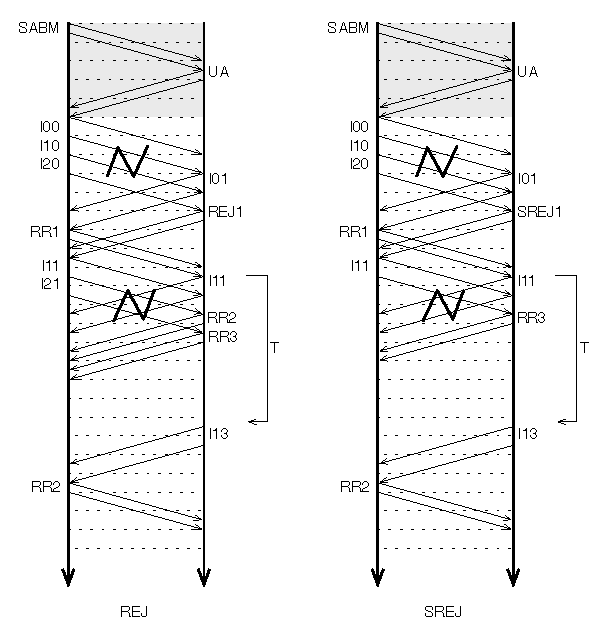
\includegraphics[scale=1.5]{Exam2009/hdlc}
\end{figure}

\setcounter{ques}{4}

\begin{ques}
	Délai de reprise le plus court : REJ car il n'y a pas besoin de réordonner les trames reçues, ce qui est la cas avec SREJ.
	
	Technique qui utilise le plus de bande passante : REJ car avec SREJ, seule la trame qui fait défaut est retransmise. Avec REJ, il faut retransmettre au plus 3 trames (ie. la largeur de la fenêtre), dont au plus 2 qui ont déjà été reçues. 
\end{ques}

\clearpage

\section{Routage} % (fold)

\begin{figure}[h!]
	\center
	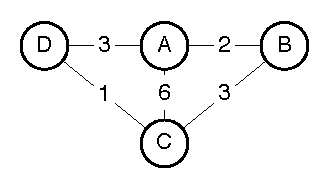
\includegraphics[scale=.7]{Exam2009/routeurs}
\end{figure}

\begin{ques}
	On a les tables de routage à la suite de la convergence : 
	\begin{figure}[h!]
		\center
		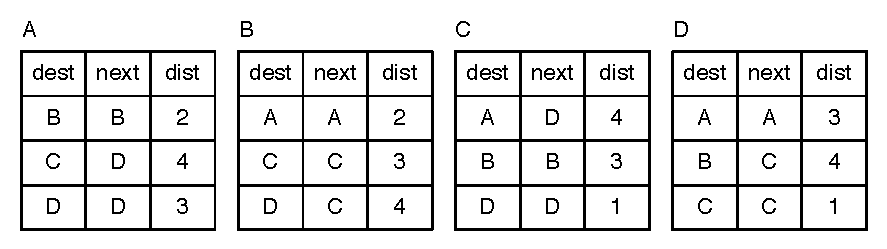
\includegraphics[scale=.7]{Exam2009/tables1}
	\end{figure}
\end{ques}

\begin{ques}
	La liaison $V_{dc}$ est rompue : 
	\begin{figure}[h!]
		\center
		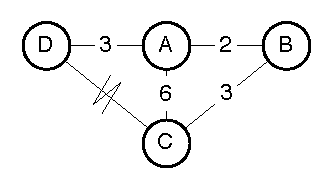
\includegraphics[scale=.7]{Exam2009/routeurs1}
	\end{figure}
	
	C et D s'en rendent compte et mettent à jour leur table de routage.\\
	On a les tables de routage : 
	\begin{figure}[h!]
		\center
		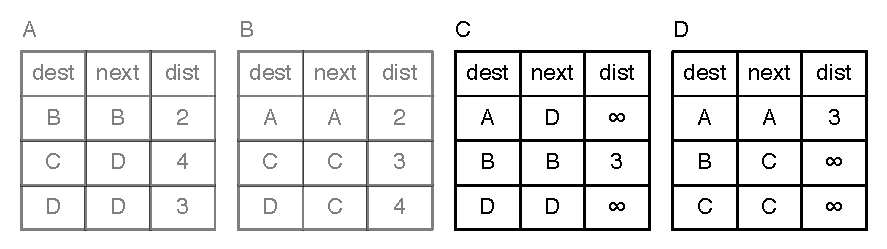
\includegraphics[scale=.7]{Exam2009/tables2}
	\end{figure}
\end{ques}

\begin{ques}
	Vecteurs de distance envoyés par C, D, A : \begin{itemize}
		\item $VC = (A\infty,\,B3,\,C0,\,D\infty)$
		\item $VD = (A3,\,B\infty,\,C\infty,\,D0)$
		\item $VA = (A0,\,B2,\,C4,\,D3)$
	\end{itemize}
\end{ques}

\begin{ques}
	Scénario d'échange :\begin{itemize}
		\item $A\leftarrow VC$
		\item $B\leftarrow VC$
		\item $A\leftarrow VD$ 
	\end{itemize}
	\begin{figure}[h!]
		\center
		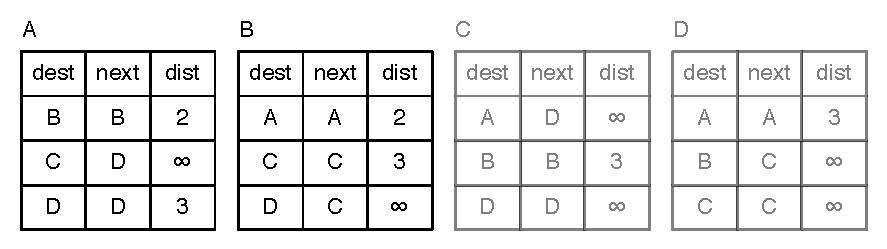
\includegraphics[scale=.7]{Exam2009/tables3}
	\end{figure}
\end{ques}
\clearpage
\begin{ques}
	Scénario d'échange :\begin{itemize}
		\item $B\leftarrow VA$
		\item $C\leftarrow VA$
		\item $D\leftarrow VA$
	\end{itemize}
	\begin{figure}[h!]
		\center
		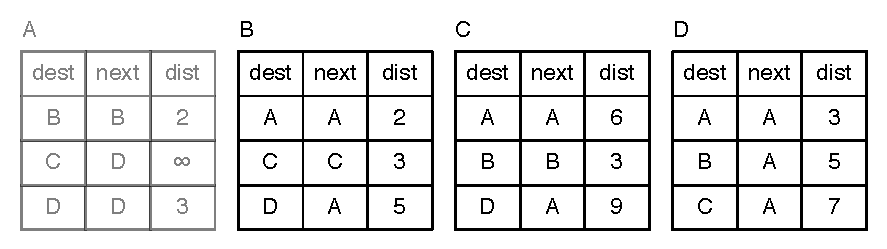
\includegraphics[scale=.7]{Exam2009/tables4}
	\end{figure}
\end{ques}

\begin{ques}
	Vecteur distance envoyé par B : $VB=(A2,\,B0,\,C3,\,D5)$
\end{ques}

\begin{ques}
	Scénario d'échange : \begin{itemize}
		\item $A\leftarrow VB$
		\item $C\leftarrow VB$
	\end{itemize}
	\begin{figure}[h!]
		\center
		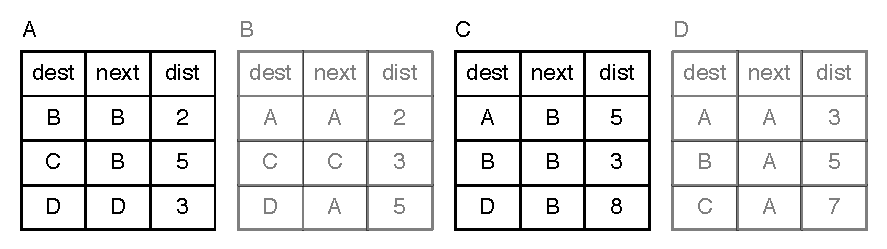
\includegraphics[scale=.7]{Exam2009/tables5}
	\end{figure}
\end{ques}

\begin{ques}
	La valeur $VA = (A0,\,B2,\,C4,\,D3)$ que A avait transmise à D était erronée. En effet, la valeur $C4$ faisait prenait en compte le lien D-C. De ce fait la distance pour aller jusqu'à C est fausse dans la table de routage de D. Il faut alors que A retransmette la bonne distance vers C à D afin qu'il actualise sa table de routage.
	
	Il faut alors que A transmette son vecteur de distances $VA=(A0,\,B2,\,C5,\,D3)$ à D.\\
	On a alors :
	\begin{figure}[h!]
		\center
		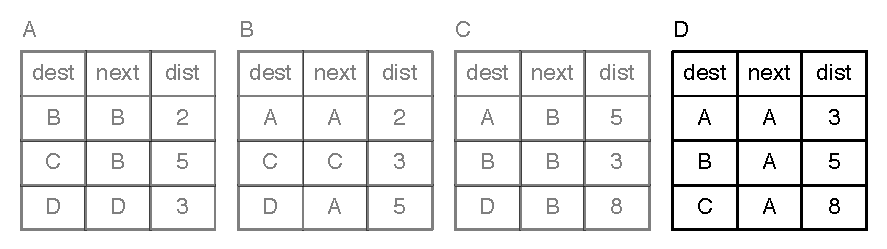
\includegraphics[scale=.7]{Exam2009/tables6}
	\end{figure}
\end{ques}
\clearpage
\section{Réseaux locaux} % (fold)

\begin{ques}
	Représentation graphique de la topologie choisie.
	\begin{figure}[h!]
	  \centering
	  \subfloat[topologie en bus]{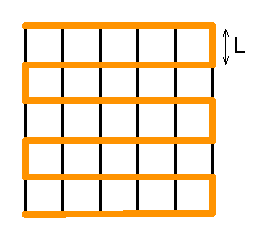
\includegraphics[width=0.25\textwidth]{Exam2009/bus}}                
	  \subfloat[Topologie en anneau]{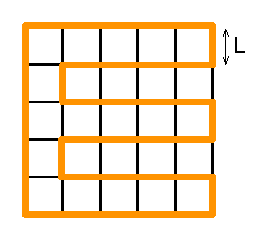
\includegraphics[width=0.25\textwidth]{Exam2009/anneau}}
	\end{figure}
\end{ques}

\begin{ques}
	Longueur de câble nécessaire :\begin{itemize}
		\item Bus : $35L$
		\item Anneau : $36L$
	\end{itemize}
\end{ques}

\begin{ques}
	Contrainte principale avec le protocole CSMA/CD si l'on veut être sûr de détecter toutes les collisions.
	
	Soit $t_{trans}$ le temps de transmission d'une trame et soit $t_{prop_{max}}$ le temps de propagation maximale d'une trame entre les deux terminaux les plus éloignés du réseau local. On a alors :\[t_{trans}\geqslant 2t_{prop_{max}}\]
\end{ques}

\begin{ques}
	Débit $D=100$ Mbit/s, $L=10$ m, vitesse de propagation $V=200\,000$ km/s, longueur d'une trame $T=512$ bits.
	
	Protocole CSMA/CD utilisable sur le réseau local construit plus haut.
	
	Calcul du temps de transmission $t_{trans}$ :\[t_{trans} = \frac{T}{D}=\frac{512}{100.10^6}=5,12.10^{-6}\;\textrm{s}\]
	
	Calcul du temps de propagation maximal $t_{prop_{max}}$ :\[t_{prop_{max}} = \frac{35\times L}{V}=\frac{35\times 10}{200\,000.10^3}=1,75.10^{-6}\;\textrm{s}\]
	
	Or $t_{trans}\geqslant 2t_{prop_{max}}$, donc le protocole CSMA/CD est utilisable sur le réseau local considéré.
\end{ques}

\begin{ques}
	Cartes réseaux qui permettent de doubler le débit pour chaque machine (ie. $D'=2D$).
	
	Calcul du temps de transmission $t_{trans}$ :\[t_{trans} = \frac{T}{2D}=\frac{512}{200.10^6}=2,56.10^{-6}\;\textrm{s} < 2 t_{prop_{max}}\]
	C'est donc impossible\dots
\end{ques}

\begin{ques}
	Résolution de ce problème : \begin{itemize}
		\item Augmenter la longueur $T$ de la trame en ajoutant des octets de bourrage. $T=700$ bits au minimum.
		\item Rapprocher les ordinateurs les uns des autres de façon à réduire la distance $L$. $L=7,31$ m max.
	\end{itemize}
\end{ques}

\section{IP} % (fold)

\begin{ques}
	Netmask du LAN1 : 255.255.255.240.\\
	Longueur du préfixe de sous-réseau : 28 car $3\times 8$ bits + 4 ($240_d=1111\,0000_b$).
\end{ques}

\begin{ques}
	Adresse IP du LAN1 : 194.215.85.160/28.
\end{ques}

\begin{ques}
	Nombre de machines que l'on peut mettre sur LAN1 : $2^4-2 = 14$. Or il y a déjà deux machines (A et R1) sur LAN1, donc on peut ajouter 12 machines sur LAN1.
\end{ques}

\begin{ques}
	Adresse de diffusion sur LAN1 : 194.215.85.175/28.
\end{ques}

\begin{ques}
	LAN2 conçu pour contenir 510 machines maximum. A cela, il faut ajouter l'adresse IP du réseau LAN2 et l'adresse de diffusion. On a alors 512 adresses IP possibles pour LAN2. Or il faut 9 bits ($log_2(512)=2$) pour coder 512 adresses différentes. De ce fait, le masque associé à LAN2 est 255.255.254.0/23.
\end{ques}

\begin{ques}
	Adresse IP de LAN2 : 131.24.64.0/23\\
	Adresse de diffusion de LAN2 : 131.24.65.255/23
\end{ques}

\begin{ques}
	Adresse IP de l'interface eth0 du routeur R1. Cette interface est connectée au réseau LAN1, donc elle a pour adresse 194.215.85.174/28.


	Adresse de l'interface eth1 du routeur R1. Cette interface est connectée au réseau LAN2, donc elle a pour adresse 131.24.6.254/23
\end{ques}

\begin{ques}
	A souhaite envoyer un message à B.\\
	Table de routage minimale de A :
	
	\begin{tabularx}{\textwidth}{XXXX}
		\toprule 
		Destination & Netmask & Gateway & Interface\tabularnewline
		\midrule
		\midrule
		194.215.85.174 & 255.255.255.240 & {*} & eth0\tabularnewline
		\midrule 
		131.24.64.12 & 255.255.254.0 & 194.215.85.174/28 & eth0\tabularnewline
		\midrule 
		default & 0.0.0.0 & 194.215.85.174/28 & eth0\tabularnewline
		\bottomrule
	\end{tabularx}
\end{ques}

\begin{ques}
	Trame Ethernet construite par A en direction de B : \begin{itemize}
		\item @MAC dest : R1 eth0
		\item @MAC source : \lstinline!5E:FF:56:A2:AF:15!
		\item @IP source : 194.215.85.168
		\item @IP dest : 131.24.64.12
	\end{itemize}
\end{ques}

\begin{ques}
	Protocole permettant à A de connaître les valeurs des adresses manquantes (ie. R1 eth0) : ARP.
	
	Le protocole ARP (\emph{Address Resolution Protocol}) permet à une machine d'obtenir l'adresse Ethernet (physique) d'une autre machine, connaissant son adresse IP (logique).
\end{ques}

\begin{ques}
	La machine A diffuse alors sur le LAN1 une trame contenant une requête ARP afin de connaître l'adresse Ethernet de l'interface eth0 du routeur R1 ayant pour adresse IP : 131.215.85.174/28
	
	Cette requête ARP aura pour adresse \lstinline!FF:FF:FF:FF:FF:FF! (adresse de diffusion) et contiendra le champ \emph{Target IP Address} égal à l'adresse IP de l'interface IP du routeur R1.
\end{ques}
\end{document}